\begin{xcs}
    A \qty{273}{K}, o argônio tem os seguintes coeficientes do virial: 
    B = \qty{-21,7}{cm^3 mol^{-1}} e C = \qty{1200}{cm^6 mol^{-2}}.
    Admitindo que a lei dos gases perfeitos seja
    suficientemente exata para estimar o segundo e terceiro termos da expansão
    (ou seja, use a lei dos gases perfeitos em caso de necessidade): 
    \begin{enumerate}[label=\alph*.]
        \item[b.] Explique como o fator de compressibilidade Z varia com a
            temperatura. Faça um esboço indicando o comportamento de Z acima e
            abaixo da temperatura de Boyle (T\(_B\)), identificando também essa
            temperatura no esboço. 
    \end{enumerate}
\end{xcs}
\begin{rsl}
    Primeiramente, deveremos explicar o que é a temperatura de Boyle. Dado um gás, conforme a sua temperatura é aumentada, a energia cinética de suas partículas aumenta, até certo ponto em que as forças atrativas entre as partículas do gás se tornam ínfimas para a descrição do comportamento do mesmo. Essa temperatura, em que as contribuições das forças atrativas e repulsivas se anulam, é denominada como temperatura de Boyle, uma forma de demonstrar a existência desse ponto, é observando que, nessa ocasião, o segundo e o terceiro coeficientes do virial se tornam zero.
    A temperatura de Boyle é muito útil na análise do fator de compressibilidade (Z) de um gás, pois ele se torna um marco para compreender o comportamento do gás, enquanto o mesmo está a uma temperatura abaixo da temperatura de Boyle, enquanto está na temperatura e enquanto está acima dela. Essa análise é possível, uma vez que, devido às propriedades da temperatura de Boyle, quando um gás se encontra na mesma fator de compressibilidade (Z) torna-se 1.  A partir da temperatura de Boyle, as forças atrativas tornam-se cada vez menos relevantes, de modo que Z pode ser apenas maior ou igual a 1 de forma estritamente crescente. Esse raciocínio está resumido na \cref{geo3b.png}, no qual o eixo X é a pressão, o eixo Y é o fator de compressibilidade (Z) e temos três curvas isotérmicas, que representam a temperatura do gás quanto à temperatura de Boyle. Comparando pontos isobáricos entre cada curva, podemos observar exatamente a relação entre a temperatura e o fator de compressibilidade.
    \begin{figure}[H]
        \centering
        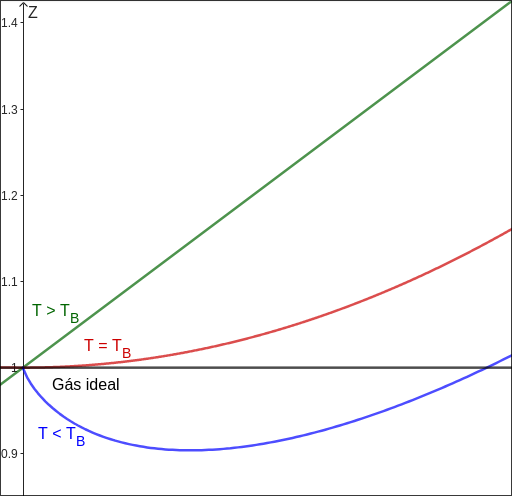
\includegraphics[width=.4\linewidth]{images/geo3b.png}
        \caption{Relação entre Z e P para curvas isotérmicas}
        \label{geo3b.png}
    \end{figure}
\end{rsl}
